%% ------------------------------------------------------------------------- %%
\section{Análise Espectral}
\label{sec:fourier}

\begin{itemize}
\item Explicar o que é um som harmônico e o modelo do sinal
\item Explicar o que é domínio do tempo e domínio de frequência e a transformada de Fourier
\item Colocar bastantes figuras: Partitura -> Som -> sinal digital (domínio do tempo) -> sinal digital (domínio da frequência) -> transcrição melódica (estimativa de F0)
\end{itemize}

\begin{figure}[h]
\centering
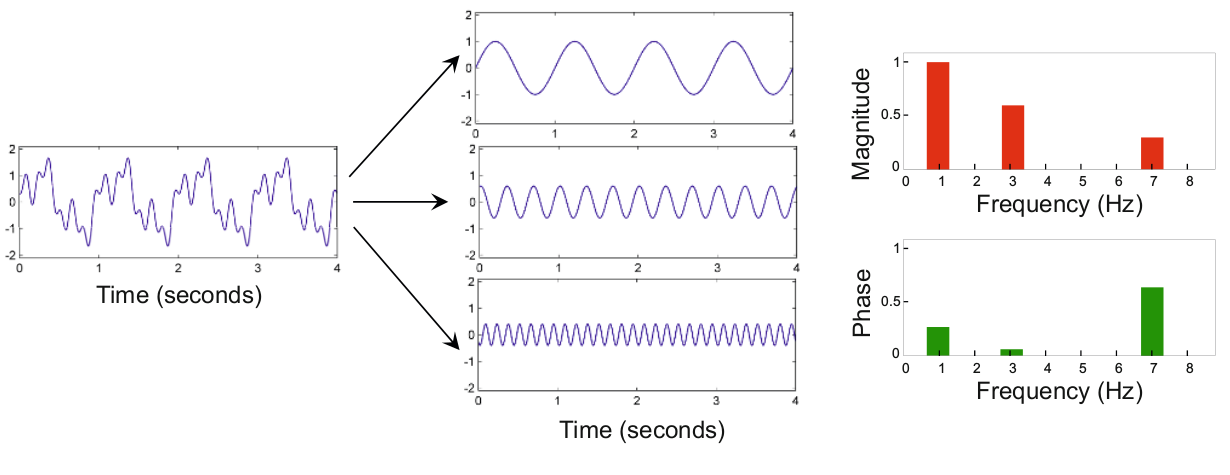
\includegraphics[width=0.6\linewidth]{figuras/fourier3}
\caption{\label{fig:fourier}Decomposição de um sinal em três parciais.}
\end{figure}

\begin{figure}[h]
\centering
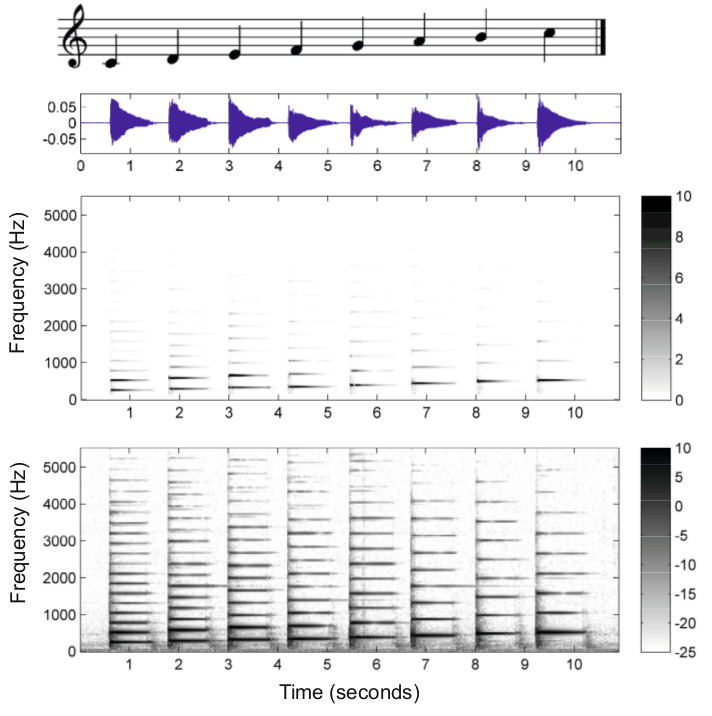
\includegraphics[width=0.6\linewidth]{figuras/fourier}
\caption{\label{fig:fourier}Transformada de Fourier em um sinal de áudio obtido a partir de um piano.}
\end{figure}